%\section{Case Study}

We additionally tested the performance of our optimization algorithm by modeling the movement of eight northern resident killer whales off the coast of British Columbia, Canada with a data set of over $5000$ dives and $80000$ depth readings. Biologgers are an essential tool used to understand the behavior of marine mammals. For example, time-depth recorders allow researchers identify and characterize dive phases, which are important for inferring behavior \citep[e.g., prey capture often occurs in the bottom phase of a foraging dive,][]{Wright:2017,Jensen:2023}. Researchers also use biologging data sets to estimate behavioral states associated with each dive \citep[e.g. foraging, resting, and traveling,][]{Tennessen:2023}. As such, we developed an HMM to identify three common dive phases (ascent, descent, and bottom) and three dive types that may indicate distinct behaviors of the animal, including resting, foraging, and traveling. We performed inference on the resulting model using our optimization algorithm in order to illustrate its computational advantages.

\subsection{Data Collection and Preprocessing}

The data used in this case study were collected in August and September of 2020 using a CATS time-depth recorder, or TDR (Customizable Animal Tracking Solutions, {\em{www.cats.is}}). Northern resident killer whales were equipped with suction-cup attached CATs tags in Queen Charlotte Sound using an adjustable 6-8m carbon fiber pole. The tags were programmed to release within 3-24 hours of attachment. Instruments were retrieved following each deploying using a Wildlife Computers 363C SPOT tag (providing Argos satellite positions), goniometer, ultra high frequency receiver and yagi antenna. The tags included 3D kinematic sensors (accelerometer, magnetometer, gyroscope), time-depth recorder, hydrophone and camera. All sensors were programmed to sample at 50 Hertz. However, for the purposes of this study, we focus on the time-depth recorder data to discern behaviorally distinct dives. We calibrated the depth readings using a MATLAB package developed by \citet{Cade:2021}, and defined a dive as any sequence of depth readings under 0.5 meters that lasted for at least two seconds. We then down-sampled the depth readings to a frequency of 0.5 Hz. The processed data set contained a total of $5858$ dives and $89462$ depth readings. Figure (\ref{fig:data}) shows the depth and change in depth for a subset of dives for one whale in the data set. 
%
\begin{figure}
    \centering
    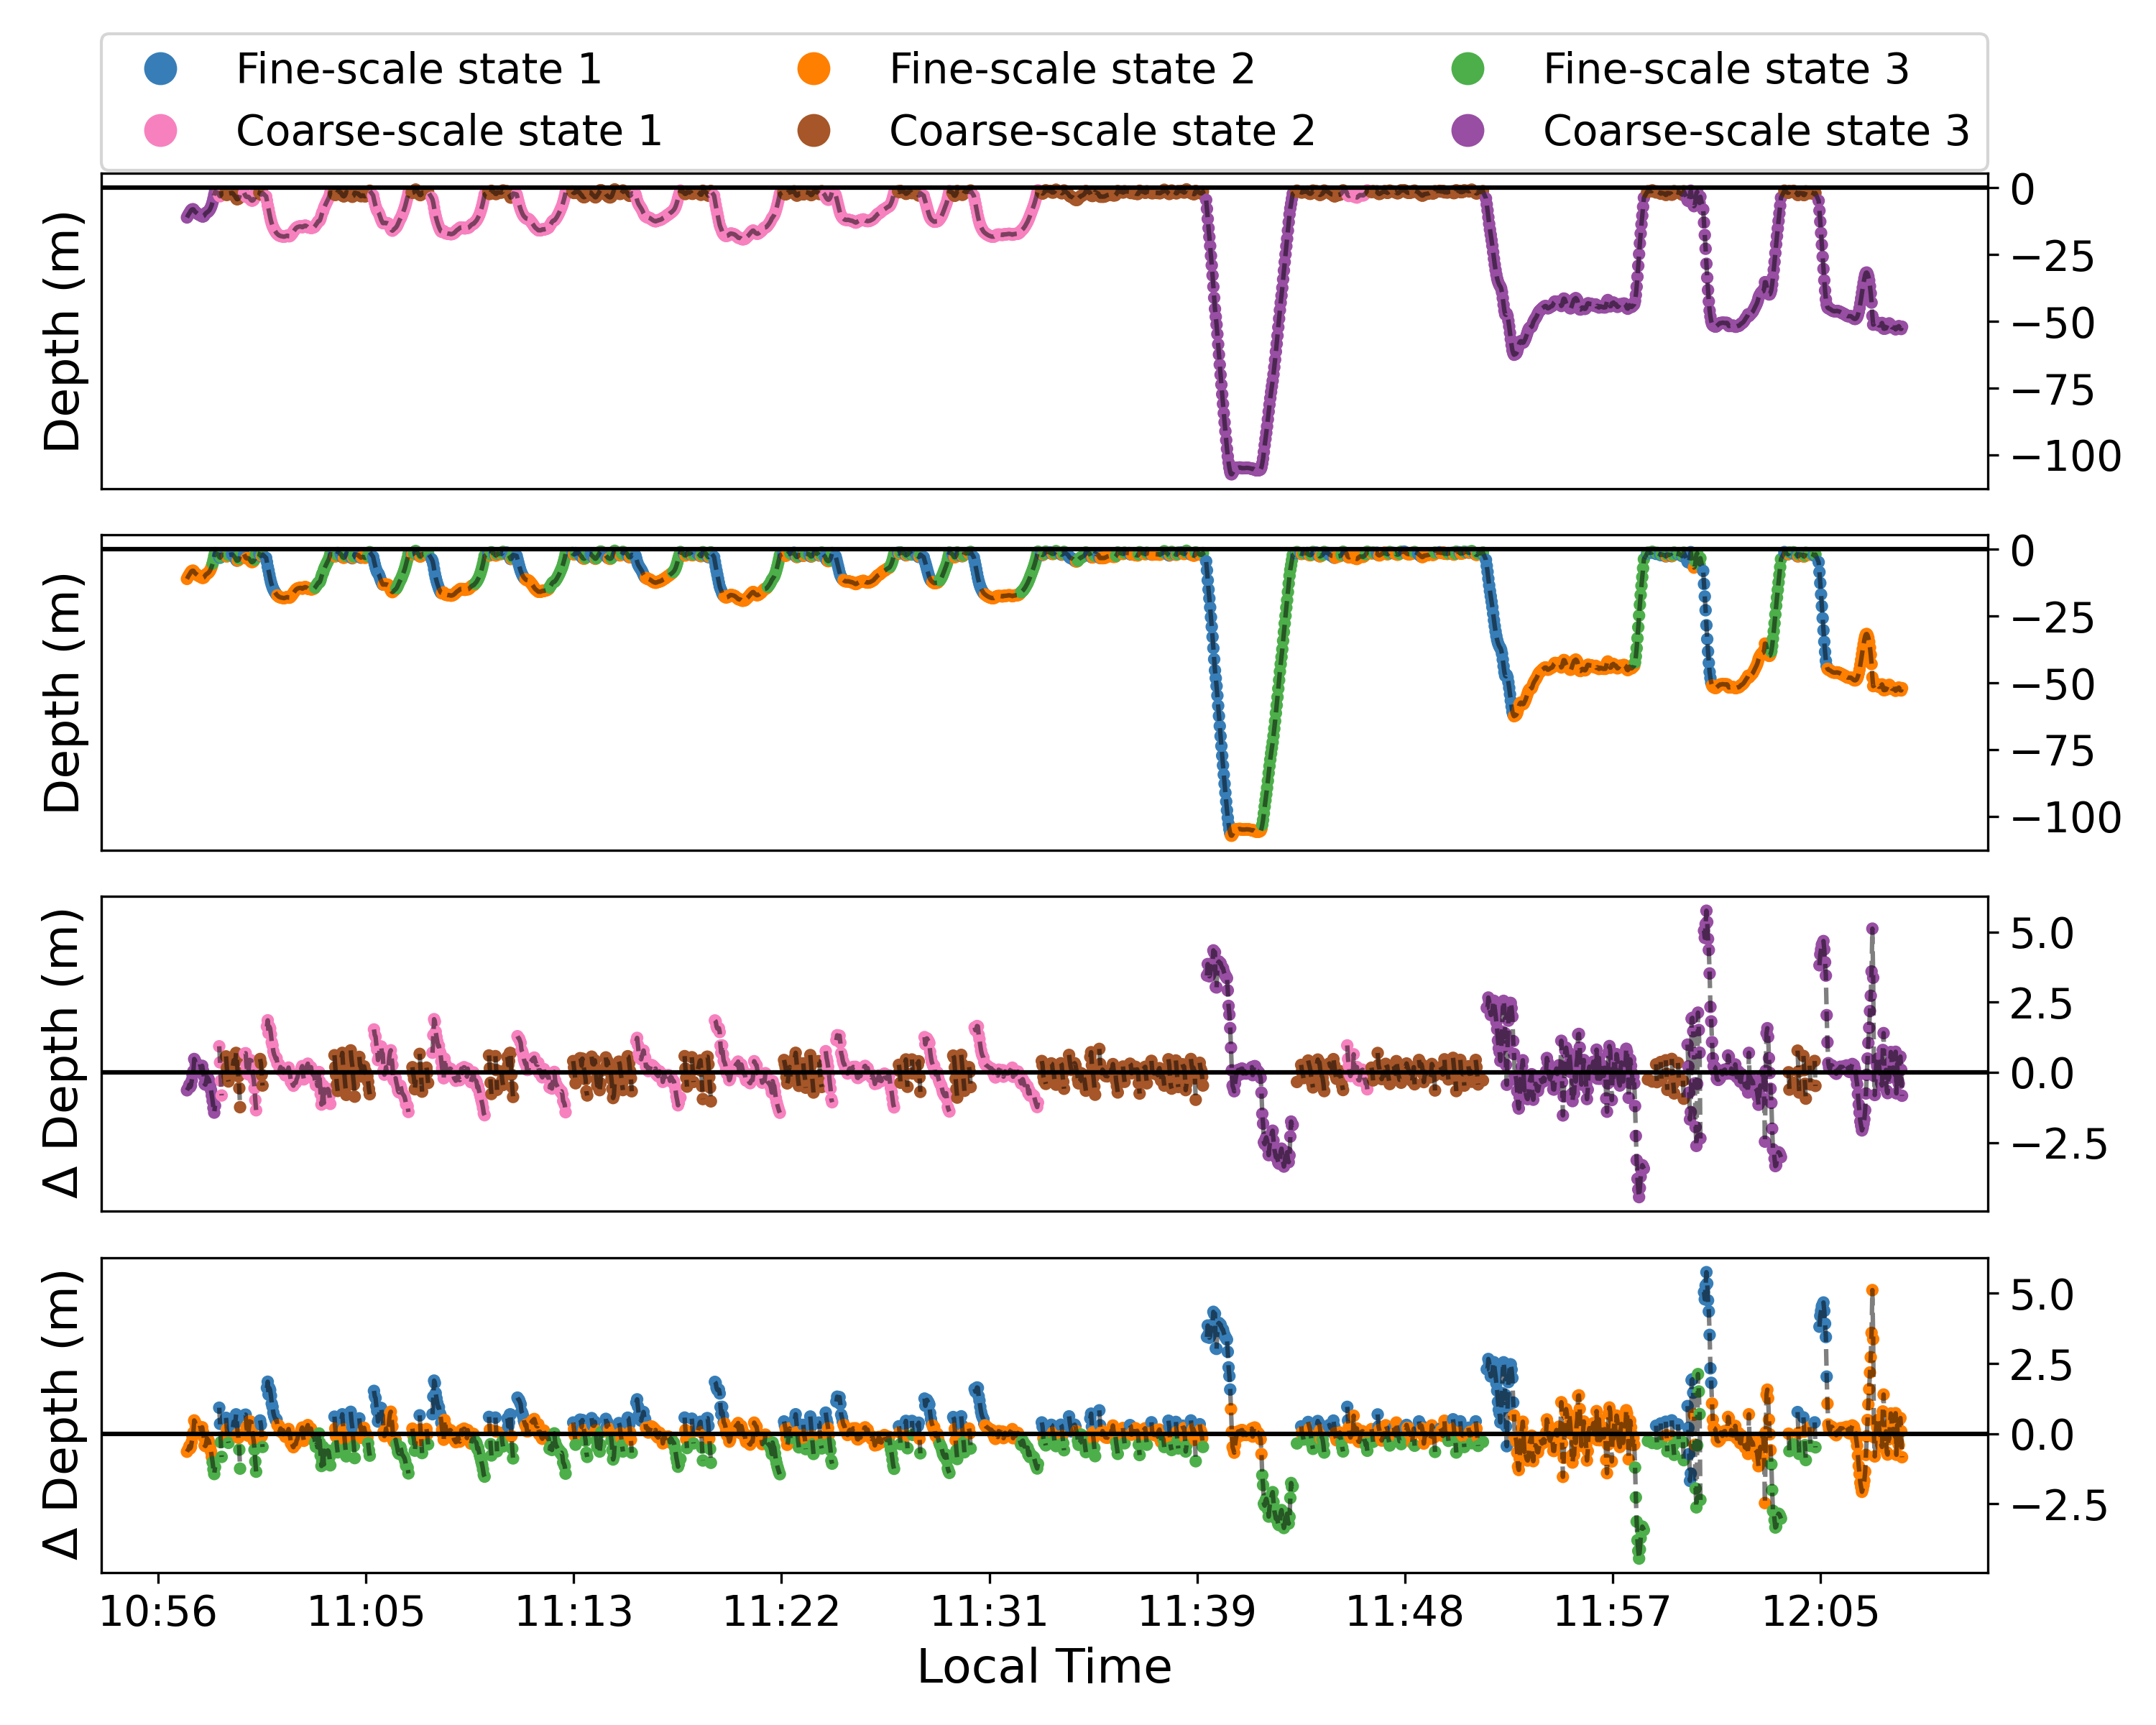
\includegraphics[width=5in]{plt/decoded_dives_kw_I107_K_3_3_nWhales_8.png}
    \caption{Depth profile and change in depth vs time of day for a selected killer whale (I107, male, born 2004) off the coast of British Columbia, Canada. The data in panels one and three are color-coded according to the most likely hidden coarse-scale state (i.e. dive type) for each dive. The data in panels two and four are color-coded according to the most likely hidden fine-scale state (i.e. dive phase) for each two-second window.}
    \label{fig:data}
\end{figure}
%
\subsection{Model Formulation}

Dive phases may vary depending upon the animal's behavior. For example, foraging dives tend to be deeper and longer than resting dives, so it is natural to model the phases of foraging dives differently compared to those of resting dives \citep{Tennessen:2019b}. As such, we used a hierarchical HMM to jointly model dive types and dive phases \citep{Barajas:2017}. Hierarchical HMMs are specific instances of traditional HMMs, so the machinery developed here is applicable to perform inference. 

We assumed there to be three dive types, which is consistent with other studies of cetaceans \citep[e.g. resting, foraging and traveling,][]{Barajas:2017}. We also assumed that there are three dive phases per dive type (descent, bottom, and ascent), which is also consistent with other studies of diving birds and mammals \citep[e.g.][]{Vivant:2014}. This resulted in a total of $N = 9$ hidden states, each corresponding to a different dive phase / dive type combination.
%
Since each dive must begin with the descent phase, we set the initial distribution $\bfdelta$ to have the form
%
%\begin{equation}
    $\bfdelta = \begin{pmatrix} \delta^{(1)} & 0 & 0 & \delta^{(2)} & 0 & 0 & \delta^{(3)} & 0 & 0 \end{pmatrix}$,
    %\label{eqn:delta_case_study}
%\end{equation}
%
where $\delta^{(i)}$ represents the probability that a killer whale begins its dive profile with a dive of type $i$. 
%
For this hierarchical HMM, we allowed the dive type to change between dives, but not within a given dive. As such, the form of transition probability matrix changed over time, so we denoted the probability transition matrix as $\bfGamma_t$. We defined a coarse-scale, inter-dive transition probability matrix $\bfGamma^{(c)} \in \bbR^{3 \times 3}$. For each dive type $i$, we also defined a fine-scale, intra-dive probability transition matrix $\bfGamma^{(f,i)} \in \bbR^{3 \times 3}$. 
%
To ensure that the dive type did not change within a dive, we defined the probability transition matrix \textit{within} a dive to have a block-diagonal form:
%
\begin{equation}
    \bfGamma_t = 
    \begin{pmatrix}
        \bfGamma^{(f,1)} & \mathbf{0} & \mathbf{0} \\
        \mathbf{0} & \bfGamma^{(f,2)} & \mathbf{0} \\
        \mathbf{0} & \mathbf{0} & \bfGamma^{(f,3)} \\
    \end{pmatrix},
\end{equation}
%
where $\bfGamma^{(f,i)}$ is upper-triangular for $i \in \{1,2,3\}$. The transition matrices were upper-triangular because the descent and bottom phases of a dive cannot occur after ascent, and the descent phase of a dive cannot occur after the bottom phase.
%
However, \textit{between} dives, we allowed the coarse-scale dive type to transition, but forced each dive to begin in the descent phase. As such, $\bfGamma_t$ took the following form:
%
\begin{equation}
    \bfGamma_t = \bfGamma^{(c)} \otimes \begin{pmatrix} 1 & 0 & 0 \\ 1 & 0 & 0 \\ 1 & 0 & 0 \end{pmatrix},
\end{equation}
%
where $\otimes$ denotes the Kronecker product.

Rather than modeling raw depth every two seconds as the observation sequence, we encoded each two-second window of depth data with summary statistics. Namely, we denoted an observation as $Y_t = \{D_t,E_t\}$, where $D_t \in \bbR$ is the change in depth in meters and $E_t = 1$ if a dive ended at index $t$ and $E_t = 0$ otherwise. 
Within dive type $i$ and dive phase $j$, we assumed $D_t$ followed a normal distribution with mean $\mu^{(i,j)}$ and standard deviation $\bfSigma^{(i,j)}$, and we assumed that $E_t$ followed a Bernoulli distribution with probability $p^{(i,j)}$. We assumed that dives must end on the ascent phase, so we set $p^{(i,1)} = p^{(i,2)} = 0$ for dive types $i = 1,2,3$. Conditioned on the dive type and dive phase, $D_t$ and $E_t$ were assumed to be independent of one another.

\subsection{Optimization Procedure}

We used a procedure similar to the simulation study to initialize the case study parameters. Let $\bar D$ denote the sample mean and $s$ denote sample standard deviation of $\{D_t\}_{t=1}^T$. We initialized the initial estimates for the mean $\left(\mu^{(i,j)}_0\right)$ and standard deviation $\left(\sigma^{(i,j)}_0\right)$ of the state-dependent density of $D_t$ as
%
%\begin{equation}
    $\mu^{(i,j)}_0 \sim \calN(\bar D, s^2)$ and $\log\left(\sigma^{(i,j)}_0\right) \sim \calN(\log(s),1)$ for $i,j = 1,2,3$,
%\end{equation}
%
where $i$ refers to the dive type and $j$ to the dive phase. Further, let $\bar E$ represent the mean of $\{E_t\}_{t=1}^T$. We initialized the state-dependent probability of observing a dive end as
%
%\begin{equation}
    $p^{(i,1)}_0 = 0$, $p^{(i,2)}_0 = 0$ and $\logit(p^{(i,3)}_0) \sim \calN(\logit(\bar E),1)$ for $i = 1,2,3$,
%\end{equation}
%
where $p^{(i,j)}_0$ is the initial estimate corresponding to the Bernoulli distribution of $E_t$ during dive type $i$ and dive phase $j$. Dive phase 3 is ascent.

Let $\bfeta^{(\bfdelta)}_k \in \bbR^3$ denote the parameters associated with $\bfdelta$ at iteration $k$ of a given optimization algorithm. The reparameterization from $\bfeta^{(\bfdelta)}_k$ to $\bfdelta_k$ is given in Equation (\ref{eqn:reparam}). We initialized the first element of $\eta^{(\bfdelta)}_0$ as zero for identifiability and the second and third elements with a standard normal distribution, $\calN(0,1)$.

Let $\bfeta_k^{(c)} \in \bbR^{3 \times 3}$ denote the parameters associated with the coarse-scale probability transition matrix at iteration $k$ of a given optimization algorithm. The reparameterization from $\bfeta_k^{(c)}$ to $\bfGamma_k^{(c)}$ is given in Equation (\ref{eqn:reparam}). We initialized the diagonal elements of $\bfeta_0^{(c)}$ as zeros, and we initialized the off-diagonal elements of $\bfeta_0^{(c)}$ with a normal distribution with mean $-3$ and unit variance, $\calN(-3,1)$.

Let $\bfeta_k^{(f,i)} \in \bbR^{3 \times 3}$ denote the parameters associated with fine-scale transition probability matrix $\bfGamma_k^{(f,i)}$. The reparameterization from $\bfeta_k^{(f,i)}$ to $\bfGamma_k^{(f,i)}$ is given in Equation (\ref{eqn:reparam}). We initialized all diagonal elements of $\bfeta_0^{(f,i)}$ as zeros and all off-diagonal elements of $\bfeta_0^{(f,i)}$ with a normal distribution with mean -1 and unit variance, $\calN(-1,1)$.

%
%If the 2-norm of the average estimated gradient $||\frac{1}{T}\sum_{t=1}^T \widehat \nabla F^{(k,m)}_t + \widehat \nabla G^{(k,m)}_t||$ ever fell below a tolerance of $10^{-8}$, we terminated the M step of algorithm and moved on to the E step. Likewise, if the relative change of the log-likelihood after one full E- and M- step of the EM algorithm ever fell below a tolerance of $10^{-10}$, we terminated the algorithm altogether. We found the ground truth MLEs by running the traditional EM algorithm until the relative change in the log-likelihood was on the order of machine precision $10^{-15}$.
%
Similarly to the simulation study, we estimated the parameters of the hierarchical HMM using our six inference algorithms ($A \in \{\text{SVRG, SAGA}\}$ and $(P,M) \in \{(\texttt{False},T),(\texttt{True},T),(\texttt{True},10T)\}$) and three baseline algorithms (BFGS, conjugate gradient, and gradient descent). All algorithms were run using 50 random initializations for a total of 12 hours each on Compute Canada Cedar nodes with 16GB of RAM.

We employed similar measures as those in the simulation study to fairly compare the optimization algorithms. In particular, we measured computational complexity in epochs rather than raw computation time and defined an epoch using the definition from the simulation study. We also estimated the maximum likelihood parameters $\bfphi^*$ for each data set / experiment pair using the same method as the simulation study. Finally, we recorded the epoch and likelihood of convergence for each optimization algorithm using the same definition of convergence as the simulation study.

\subsection{Case Study Results}

Our model predicted dive phases and dive types that are in line with previous studies of marine mammal diving behavior. For example, dive types are separated by shallow, medium, and deep depths, which is similar to results from \citet{Barajas:2017}. Further, each dive has a well-characterized bottom phase that occurs at approximately 70\% of the maximum depth for all dive types. This finding is similar to the results from \citet{Tennessen:2019a}. See Figure (\ref{fig:data}) and supplement B for further detail.
%This section focuses on results from the optimization procedure rather than the parameter estimates and decoded dive types / dive phases. For parameter estimates and decoded dive phases, see Supplement B.

Most importantly, this case study demonstrates that all of our stochastic algorithms converged in fewer epochs and to regions of higher likelihood compared to the full-batch baselines; see Figures (\ref{fig:ll_trace_case}--\ref{fig:scatterplot_case}).
%
\begin{figure}[h]
    \centering
    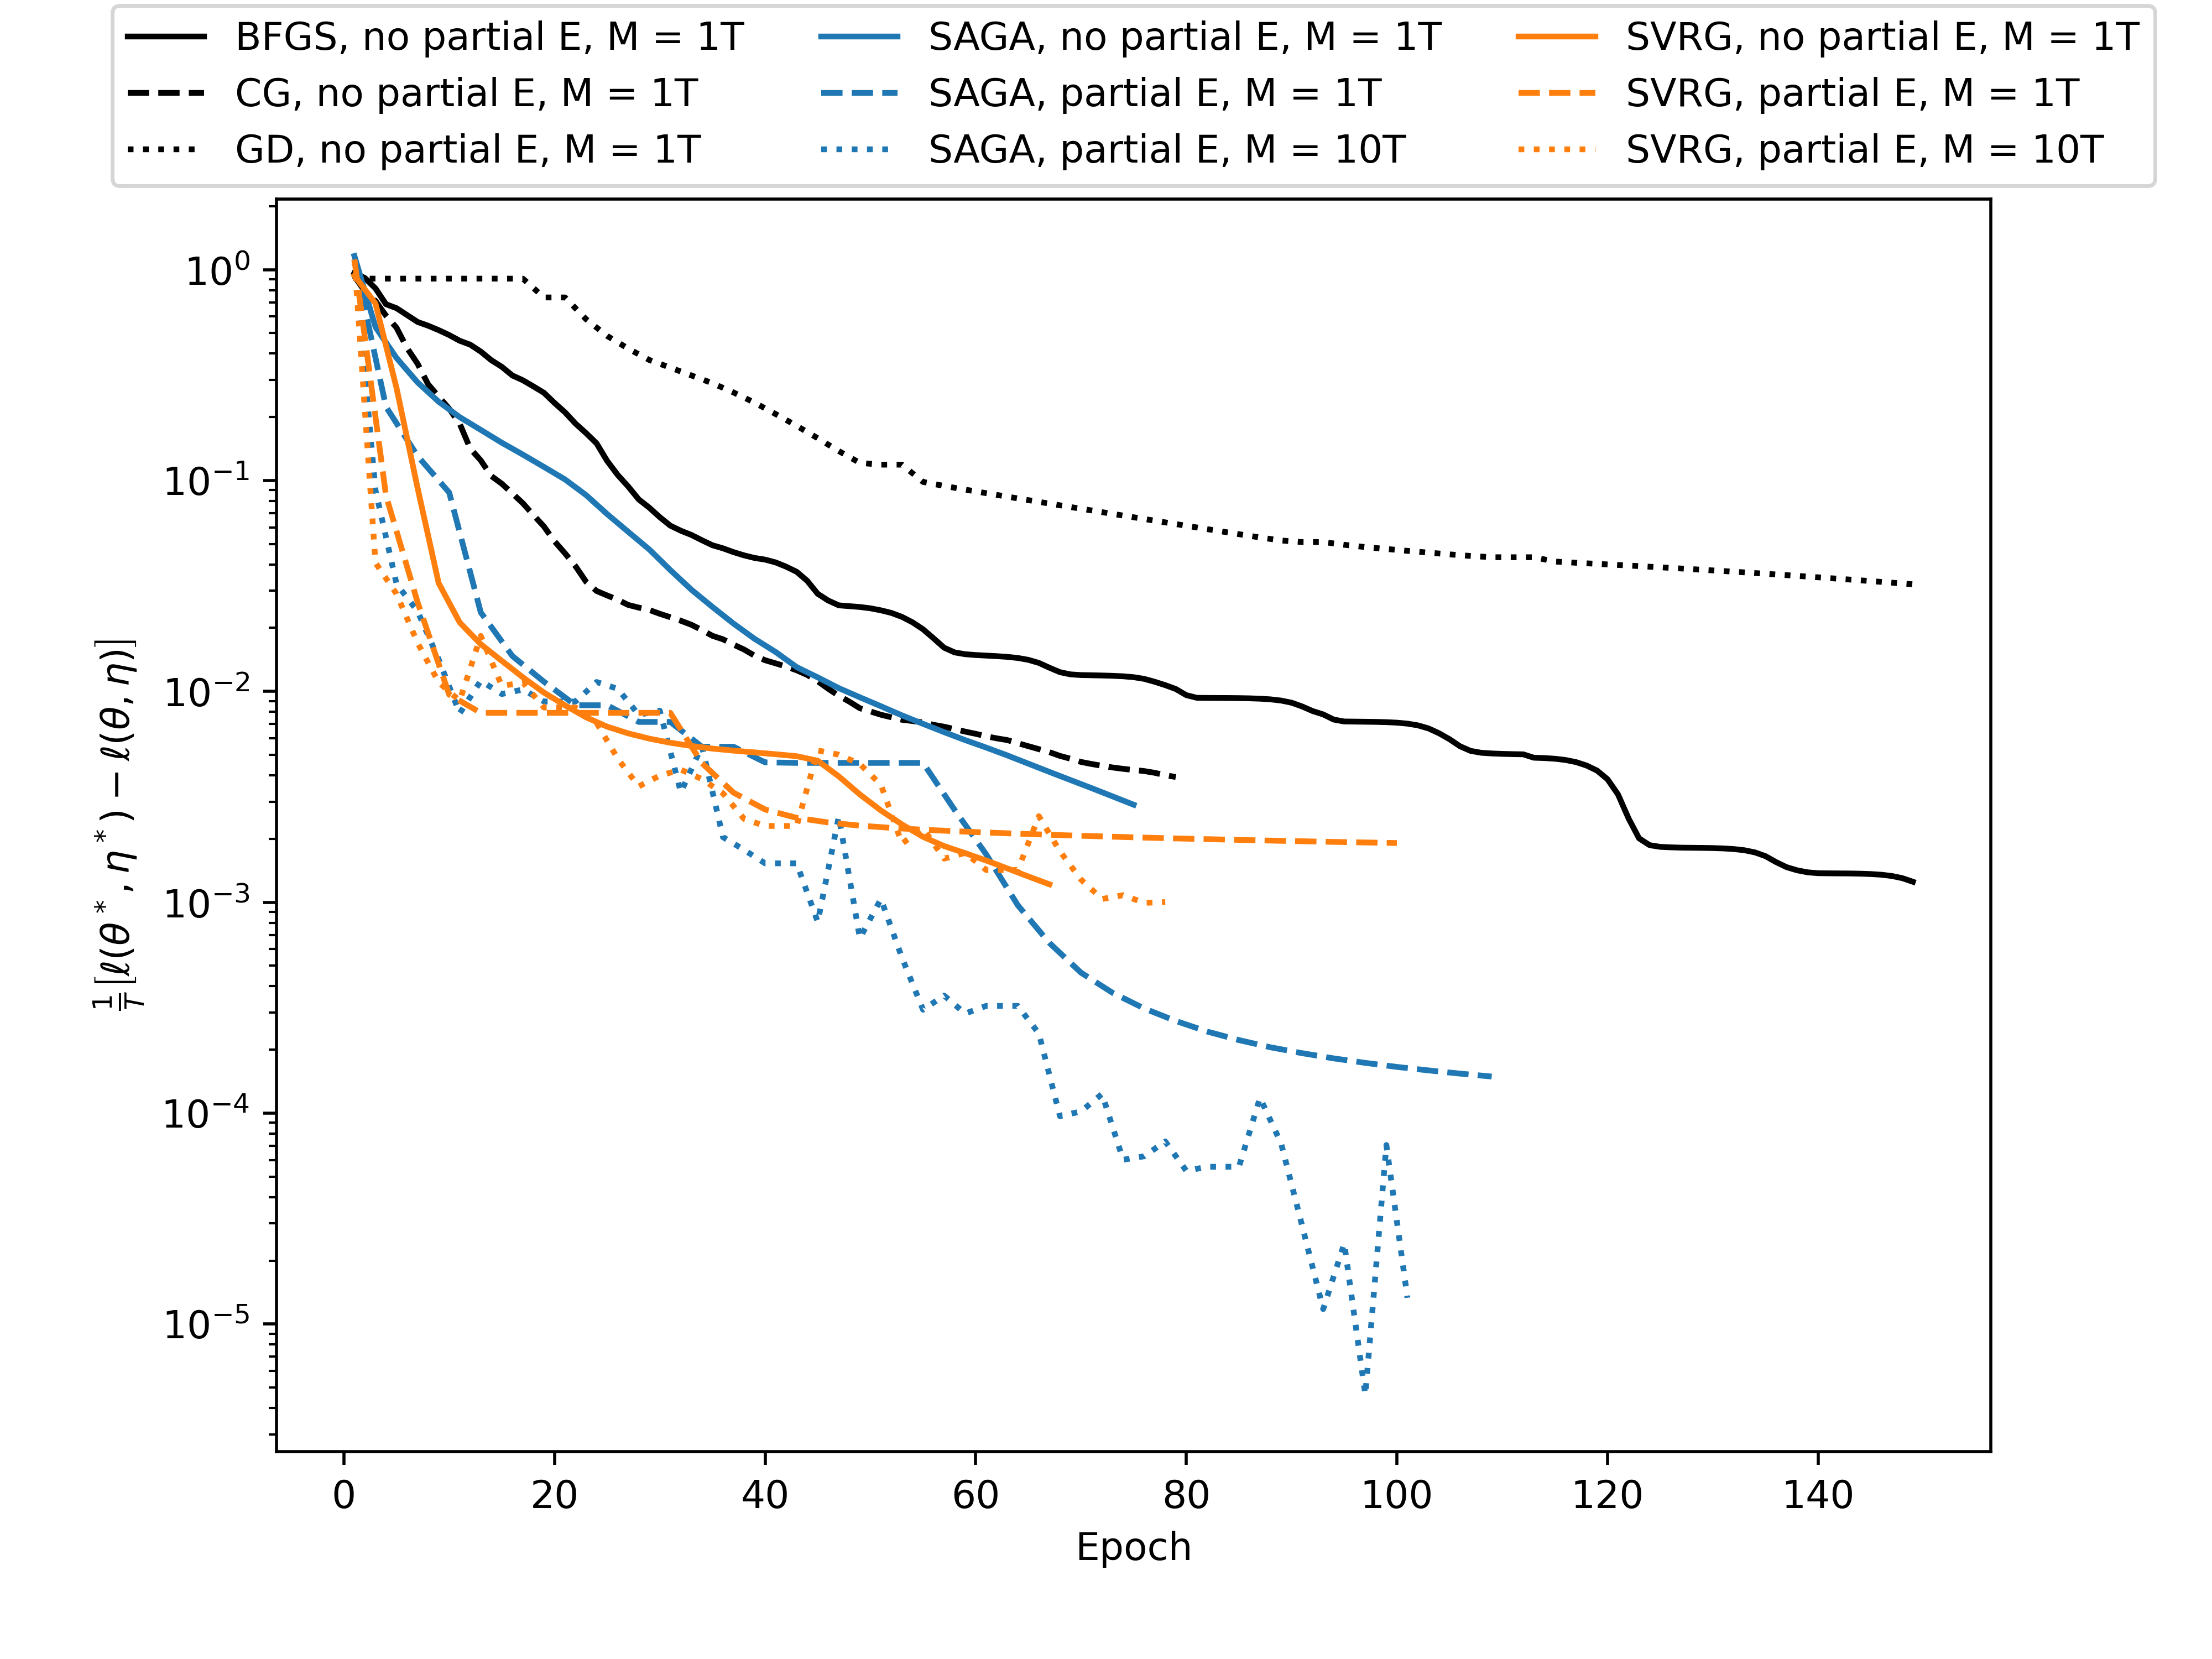
\includegraphics[width=4in]{../plt/log-like_v_epoch_K-3-3.png}
    \caption{
    Maximum log-likelihood minus log-likelihood (all over $T$) vs epoch for 12 hours or 100 epochs (whichever came first) for the HMM from the killer whale case study. FE corresponds to $P = \texttt{False}$, and PE corresponds to $P = \texttt{True}$. The log-likelihood of $\bfphi$ is denoted as $\ell(\bfphi)$ on the y-axis, which is on a log-scale. We display the random initialization of each algorithm that resulted in the highest likelihood after 12 hours. Dots correspond to the epoch and likelihood at convergence for each algorithm.
    }
    \label{fig:ll_trace_case}
\end{figure}
%
\begin{figure}[h]
    \centering
    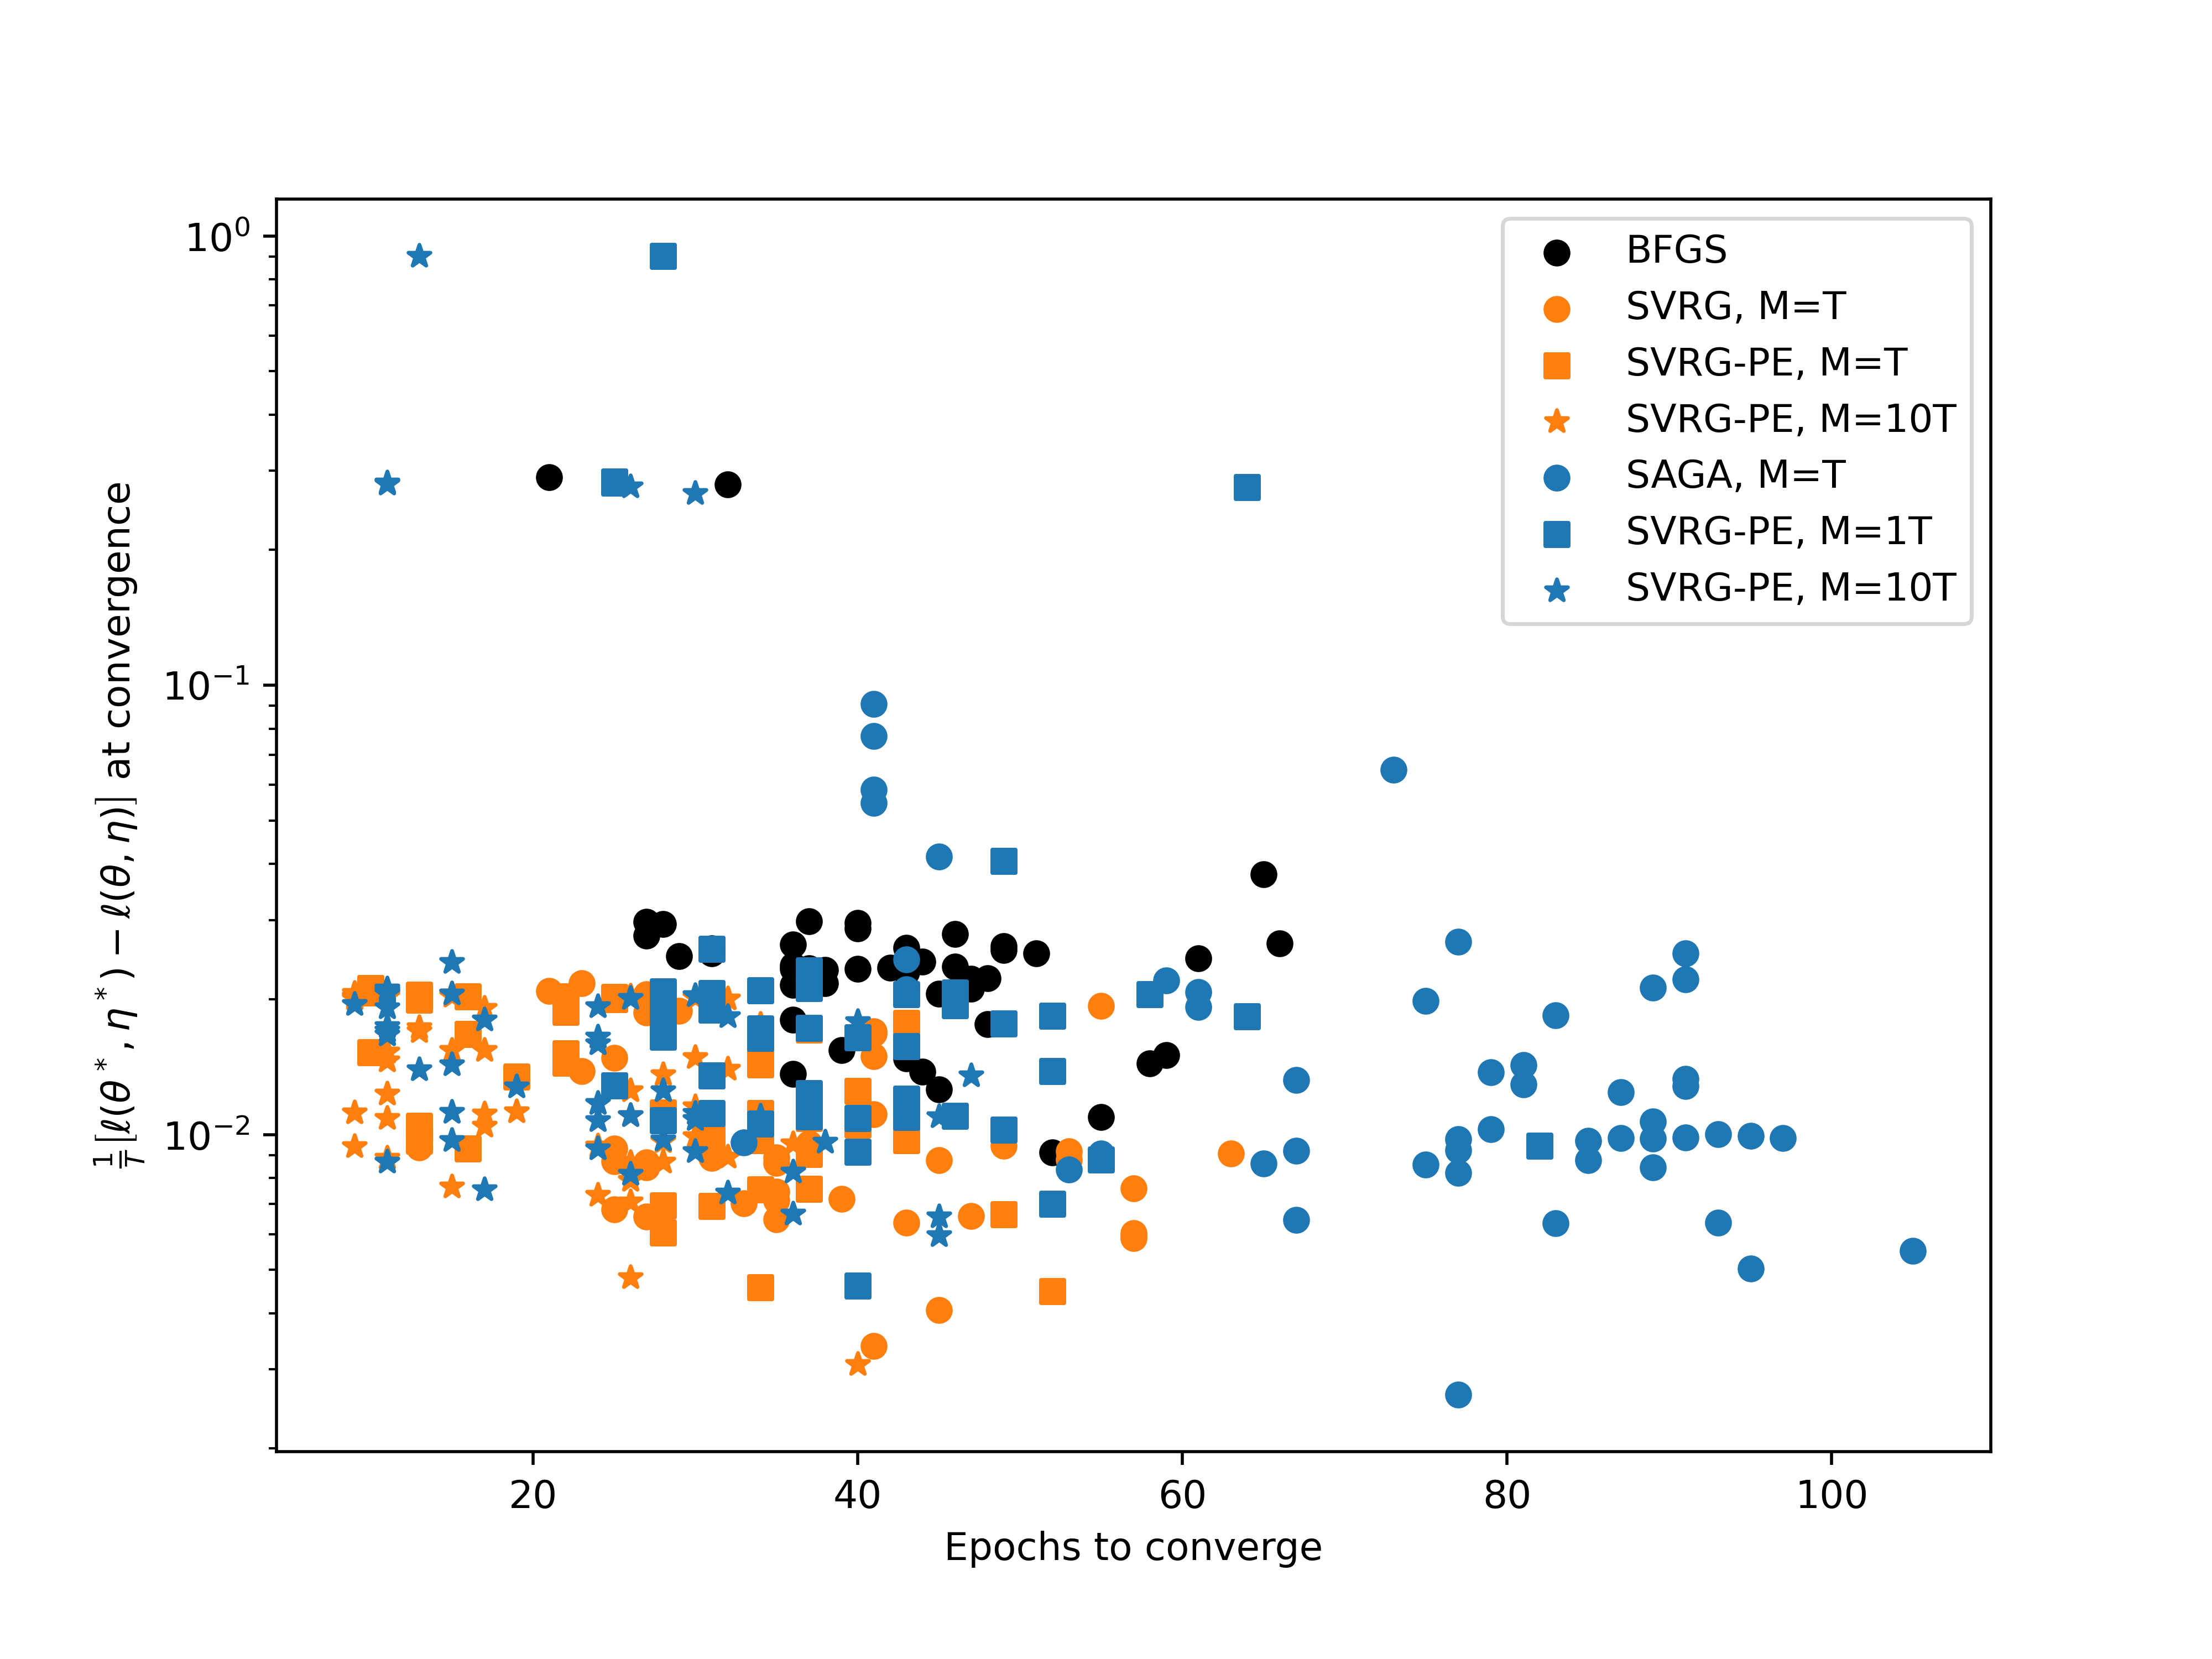
\includegraphics[width=4in]{../plt/scatterplot_case_study.png}
    \caption{Maximum log-likelihood minus log-likelihood at convergence (all over $T$) versus epochs to converge for the killer whale case study. FE corresponds to $P = \texttt{False}$, and PE corresponds to $P = \texttt{True}$. The log-likelihood of $\bfphi$ is denoted as $\ell(\bfphi)$ on the y-axis, which is on a log-scale.}
    \label{fig:scatterplot_case}
\end{figure}
%
All algorithms occasionally converged to sub-optimal local minima, but Algorithm (\ref{alg:EM-VRSO}) with $A = \text{SVRG}$ and $P=\texttt{True}$ and $M=T$ tended to converge in the fewest epochs to regions of highest likelihood; see Figure (\ref{fig:scatterplot_case}). As with the simulation study, Algorithm (\ref{alg:EM-VRSO}) with $A = \text{SVRG}$ tended to converge in fewer epochs compared with $A=\text{SAGA}$; see Figure (\ref{fig:ll_trace_case}). Setting $P = \texttt{True}$ appears to be of particular use early in the optimization procedure (i.e the first $\approx$ 5 epochs, see Figure \ref{fig:ll_trace_case}). This behavior is intuitive because the proper weights $\left(\bfgamma(\bfphi_k^{(m)}) ~ \text{and} ~ \bfxi(\bfphi_k^{(m)})\right)$ change rapidly early in the optimization procedure. 

%All of the algorithms presented in this paper converge with higher likelihood than BFGS (on average), and all algorithms except for algorithm (\ref{alg:P-EM-SO}) with SAGA tend to converge in fewer epochs than BFGS.

%Figure (\ref{fig:scatter_case}) displays scatter plots of the number of epochs to converge and the loss at convergence of each algorithm vs. BFGS for the same data set and parameter initializations.
%
%\begin{figure}
%    \centering
%    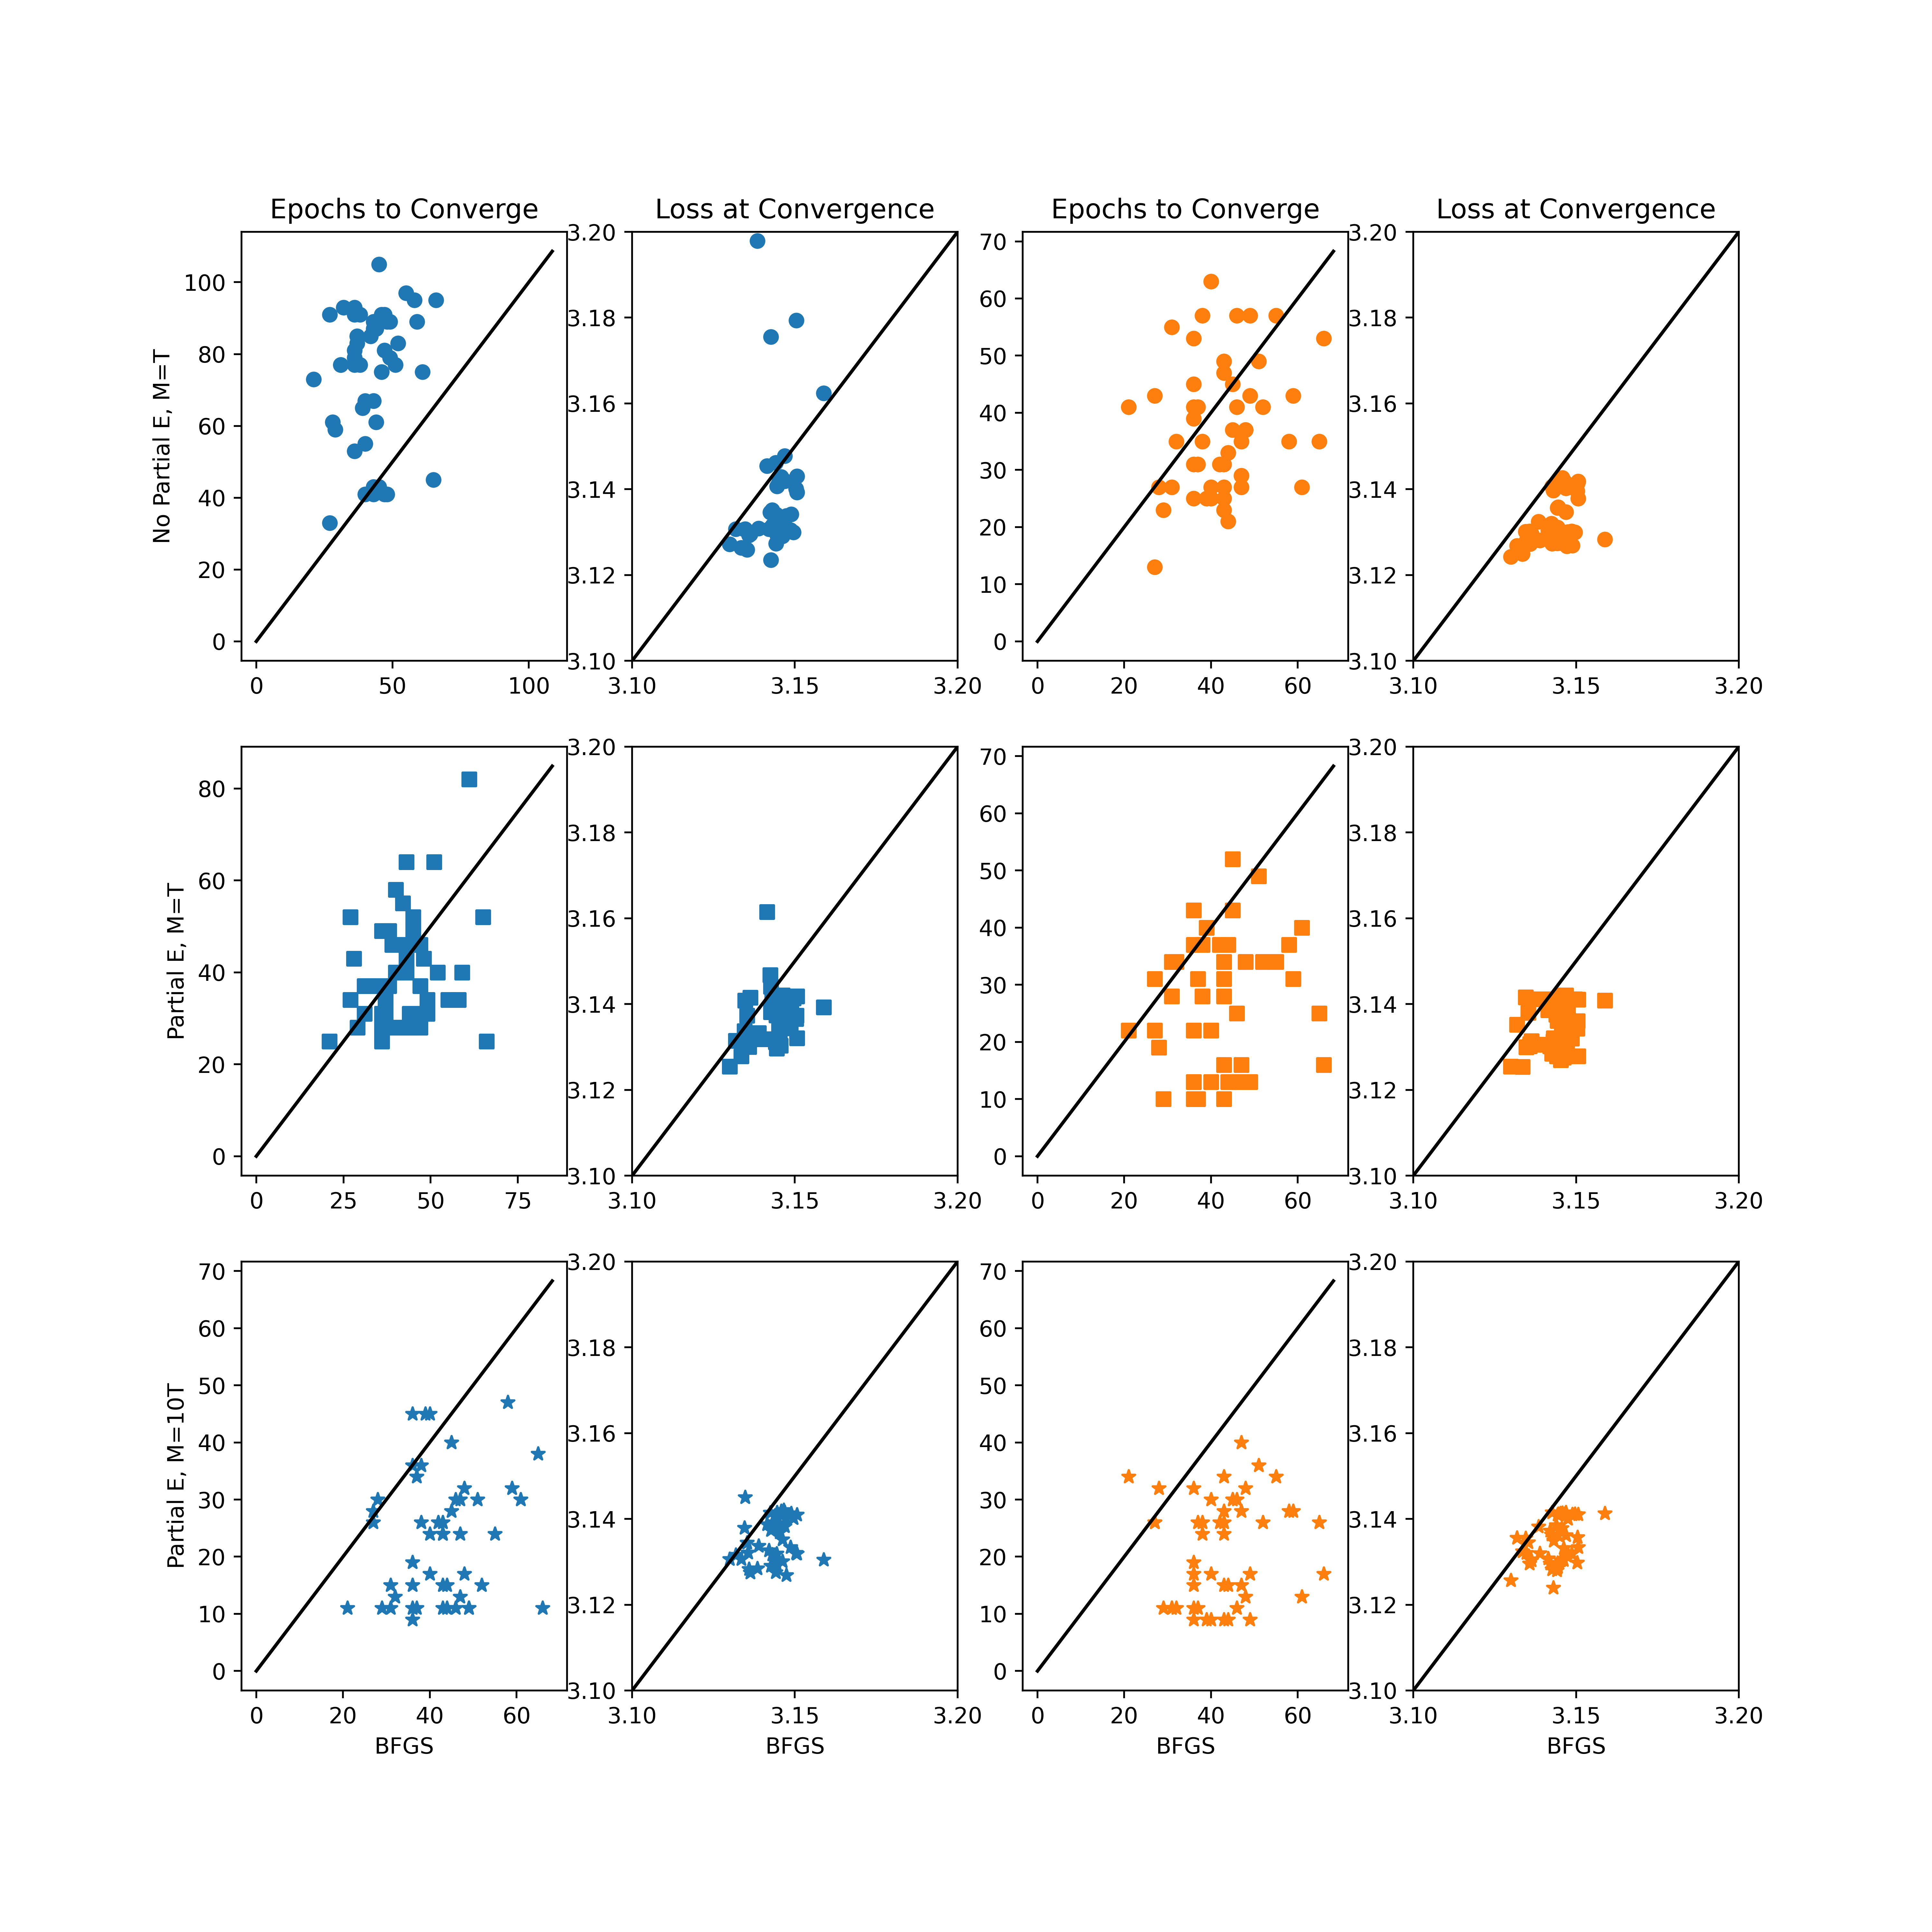
\includegraphics[width=6.5in]{../plt/paired_scatter_case_study.png}
%    \caption{Number of epochs to converge (columns 1 and 3) and the loss at convergence (columns 2 and 4) of each algorithm vs. BFGS for identical data sets and parameter initializations. Lower is better for both criteria, so data points below the line $y=x$ suggest that the stochastic optimization algorithms perform better.}
%    \label{fig:scatter_case}
%\end{figure}
%

%SAGA without a partial E step performs similarly to the EM algorithm in a per-epoch basis because SAGA is successfully converging for the M step when $M = T$. However, it does not perform as well as the EM algorithm on a per-time basis because the M step is significantly slower when using SAGA vs the closed-form solution. This behavior is expected, and SAGA has a significant advantage over the EM algorithm in that it only requires gradients rather than sufficient statistics.

%mplementing a partial E step shows that SAGA can outperform the EM algorithm when the parameter estimates are far from the optimal solutions and when the underlying HMM does not mix rapidly. This is likely because the weights of the $F$ and $G$ are very inaccurate at first, and updating them early in the optimization procedure yields a significant speed-up. In addition, if the Markov chain is rapidly mixing, then updates to $\gamma_{t_m}$ and $\xi_{t_m}$ at a single data point are more accurate. Future work may involve performing the partial-E step for many weights at once sequentially, depending upon the mixing time of the current estimate of $\eta_k$.